%% ------------- Portuguese version ------------ 
\documentclass[portuguese]{sbrt} 
\usepackage[portuguese]{babel} 
\usepackage[utf8]{inputenc} 
\newtheorem{theorem}{Theorem} 
\usepackage[T1]{fontenc} 
\usepackage[pdftex]{hyperref} 
\usepackage{graphicx,url} 
\usepackage[hang]{subfigure} 
\usepackage{psfrag} 
\usepackage{comment} 
\usepackage{graphicx}
\usepackage{amsmath}
\graphicspath{ {./images/} }
%% --------------------------------------------- 
  
%% If writing in English, remove the lines above 
%% and uncomment the lines below 
  
%% ------------- English version --------------- 
%\documentclass[english]{sbrt} 
%\usepackage[english]{babel} 
%\usepackage[utf8]{inputenc} 
%\newtheorem{theorem}{Theorem} 
%% --------------------------------------------- 
  
\begin{document} 
  
\title{Projeto Final GCC253 - Auto Calibração de Câmeras em Visão Estéreo} 
  
\author{Gabriel Martins Silva, Lucas Hideki Sekiya Nascimento, Valter Granato Neto, Vanessa Luana Soares Corrêa. 
\thanks{\centering \textbf{\textit{Complexidade e Pojeto de Algorítmos} -- \today \\ Prof. Douglas H. S. Abreu}}% 
} 
  
\maketitle 

  
\markboth{Projeto Final GCC253 - Complexidade e Projeto de Algorítmos - Departamento de Ciência da Computação (DCC) - Instituto de Ciências Exatas e Tecnológicas (ICET)- UFLA - 2022/1}{} 
  
  
%% If writing in English, remove both 'resumo' and 'chave' 
%% ------------- Portuguese version ------------ 
  
\begin{resumo} 
%\textit{Reduzir, pois o resumo deve conter no máximo 100 palavras.}  
O presente trabalho tem como objetivo estudar alguns métodos de auto-calibração para câmeras utilizadas em visão estéreo. A visão estéreo trabalha com a reconstrução da informação tridimensional de ambientes a partir de imagens capturadas por câmeras com campo de visão sobreposto. Uma vez que esse processo se baseia em captura de imagens, é necessário que as câmeras estejam devidamente calibradas para garantir a confiabilidade e precisão desse método
\end{resumo} 
\begin{chave} 
algoritmos, complexidade, visão computacional, câmeras digitais, revisão bibliográfica, calibração. 
\end{chave} 
  

%% --------------------------------------------- 
  
  

\section{Introdução} 
\label{sec:introducao} 
  
Dentro da computação, a visão estéreo é a área que estuda a reconstrução de dados tridimensionais a partir de imagens bidimensionais \cite{MadalenaMenotti:2020}. Esse tipo de visão está presente em diversos animais - em geral predadores - e baseia-se na comparação de duas imagens parecidas, porém com um pequeno deslocamento: cada olho capta uma imagem levemente diferente do outro. Essas imagens são processadas pelo cérebro e o animal, a partir das imagens bi-dimencionais captadas pelos olhos, consegue atribuir a noção de profundidade ao ambiente que está sendo visualizado.

\newline
Assim como nesses animais, a visão estéreo na computação passa pelas etapas de coleta de imagens e processamento: duas ou mais câmeras captam imagens de um mesmo ambiente, porém de posições diferentes. As imagens são analisadas e a partir delas pode-se recuperar informações tridimensionais daquele ambiente.
 
\newline
Essa concepção também é aplicada em projetos de realidade virtual para causar a ilusão de profundidade e tridimensionalidade, como podemos ver na figura 1
\begin{wrapfigure}
    \begin{center}
        \centering
	    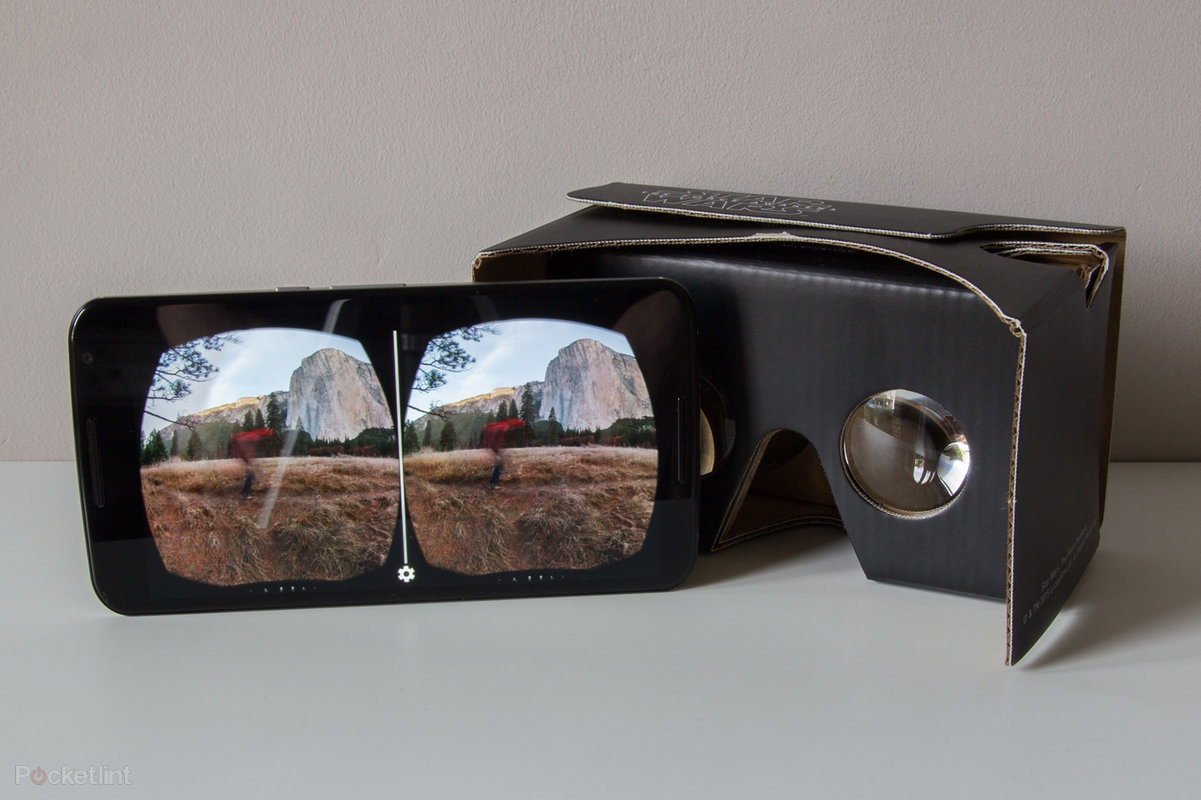
\includegraphics[scale=0.8]{vr}
	    \caption{Figura 1: Implementação de visão estéreo em óculos de realidade virtual}        
    \end{center}
\end{wrapfigure}

\newline
Tendo como base duas câmeras das quais se sabe a posição e o direcionamento, é possível calcular a posição de qualquer ponto dentro do campo de visão dessas câmeras, desde que esse ponto esteja em uma área sobreposta dentro dos campos de visão. Para calcular a posição do ponto é utilizada triangulação, é possível  verificar na figura 2

\begin{wrapfigure}
    \begin{center}
        \centering
	    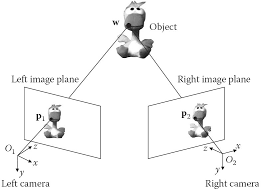
\includegraphics[scale=1.0]{triangulação}
	    \caption{Figura 2: triangulação de um ponto a partir de imagens sobrepostas na visão estéreo}        
    \end{center}
\end{wrapfigure}

\newline
A visão estéreo é largamente utilizada em sistemas de monitoramento, uma vez que possui uma alta precisão e seu custo de implementação é relativamente baixo. Entretanto, faz-se necessário um processo de calibração para garantir a precisão e qualidade desses sistemas. A auto-calibração é realizada utilizando capturas de cenas estáticas, se que se altere os parâmetros intrínsecos da câmera, dispensando o uso de objetos conhecidos previamente.

\newline
Este artigo se encontra organizado da seguinte forma: na seção II são descritos os parâmetros intrínsecos e extrínsecos das câmeras ~\ref{sec:parametros}. Na seção III são expostos os métodos de calibração propriamente ditos ~\ref{sec:metodos}. Na seção IV discute-se o desempenho dos métodos descritos na seção III ~\ref{sec:desempenho}. Na última seção são retomados os principais pontos abordados ao longo do artigo~\ref{sec:conclusao}.
 

\section{Parâmetros intrínsecos e extrínsecos}
\label{sec:parametros}
Os parametros necessários para realizar os calculos de calibração das camêras foram separados em dois grupos nomeados como parametros intrínsecos e extrínsecos. Sendo intrínsecos sendo referentes a paramêtros internos da camêra fotográfica, e extínsecos externos a camêra e especificamente aos dados da foto digital.

\newline
Lista de parametros intrínsecos:
\begin{itemize}
    \item • Distância focal: A distância focal em pixels.
    \item • Ponto principal: coordenadas do ponto principal.
    \item • Coeficiente de inclinação: define o ângulo entre os eixos x e y do pixel.
    \item • Distorções: coeficientes de distorção de imagem (radial e tangencial).
\end{itemize}

\newline
Lista de parametros extrínsecos:
\begin{itemize}
    \item • Rotação: Um conjunto de matrizes de rotação 3x3
    \item • Translação: Um conjunto de vetores 3x1.
\end{itemize}

Fazendo parte da configuração e preparação para a execução dos algoritmos de calibração, é considerada um \textit{grid} com conjunto de coordenadas \{\mathrm{X,Y,Z}\} e uma matriz \textit{A} que representa a matrix intrínseca da câmera.
  $$
  A =
  \begin{bmatrix}
   \alpha & \gamma & u_{0}\\ 
   0      & \beta  & v_{0}\\
   0      & 0      & 1    
  \end{bmatrix}
  $$
\newline
  Na definição das variáveis ($u_{0}, v_{0}$) são as coordenadas do ponto principal e $\alpha$ e $\beta$ são os fatores escalares na imagem sobre os eixos u e v. $\gamma$ representa o parâmetro de assimetria dos dois eixos.
\section{Métodos de calibração}
\label{sec:metodos}

A maioria dos metodos de calibração existentes são baseados em algoritmos de
calibração manual off-line para alvos ou padrões de referencia especificos
O foco do nosso estudo está relacionado aos métodos tradicionais de calibração
O método de calibração tradicional pode calibrar com precisão os parâmetros da câmera
utilizando alvos planos ou estéreos. 

Métodos de modelo planar
Esse metódo tem sido amplamente estudado por Zhang \cite{Zhang:2000} propôs calibrar a câmera com um tabuleiro de xadrex.
A câmera é necessária para visualizar o padrão quadriculado exibido em várias direções
na qual deve identificar seus cantos em uma imagem e calcular toda a divisão do tabuleiro. 
Com isso se tiver qualquer valor errado ou canto não detectado, insere no parâmetro de calibração o erro encontrado e uma nova calibração é feita.

Métodos de calibração baseados em objetos 3D
Esse metodo simplifica o procedimento de calibração ao colocar o alvo no campo de visão da câmera uma vez que para obter os parâmetros de calibração.
Su et ai \cite{Svoboda:2005}usaram um objeto de calibração esférica como padrão de referência especializado para calibrar os parâmetros geométricos entre qualquer número de câmeras testadas 
Para realizar pode-se utilizar um ponto brilhante ou um ponto em que se destaque e esteja presente em todas as câmeras, para que a imagem seja reconstruída
Para utilizar o método proposto por Su et al \cite{Svoboda:2005}, é necessário somente a matriz de dados W contendo os pontos da imagem.
Este tipo de método gera resultados muito precisos, porém depende dos pontos diferentes que essa matriz irá conter
Após a obtenção dessa matriz, procura-se os pontos semelhantes nas outras matrizes, o que é chamado de correspondência.


\section{Desempenho} 
\label{sec:desempenho}
observando os algoritmos de:
* normalização:: que tem como objetivo de transformar o mapeamento das coordenadas da imagem invertida
* inicialização da calibração dos parâmentros:: que consiste na coleta de dados camera, e configura de tal maneira que prepare para o algoritmo de otimização da calibração, buscando assim melhores condições de bons resultados do algoritmo.
* otimização a não linear:é onde realmente é executado o algoritmo de calibração utilizando as otimizações feitas pelo preparo e tratamento prévios dos parâmetros.

\section{Analise de complexidade}
\label{sec:analise_complexidade}
Presente no artigo, o autor faz referência a dois trabalhos\ref{Zhang:2000} em que a analise de complexidade se dá em uma complexidade de $f(n) = 2O(n)$ e no trabalho[5]\ref{Svoboda:2005} a complexidade obtida foi de $f(n) = 100O(n^2)$ o que demonstra menos complexidade e melhores soluções nos dois primeiros trabalhos citados do que no terceiro. Nas palavras do autor do artigo, descreve de forma resumida as duas abordagens de diferentes complexidades na seguinte forma: "O método proposto por Zhang [3], [4] efetua a calibração
individual da câmera usando a detecção de cantos em uma
imagem planar. Utilizou-se para exemplificar o uso deste
método imagens de um tabuleiro de xadrez.
Svoboda et al. [5] propôs a calibração de sistemas multi-
câmeras usando a detecção de um ponto principal em uma
sequência de imagens, onde este ponto tem que ser comum
em todas as imagens." \ref{MadalenaMenotti:2020}
\section{Conclusão}
\label{sec:conclusao}


\bibliographystyle{plain} 
\bibliography{ref}

\end{document} 
